% !TeX encoding = UTF-8
% !TeX spellcheck = de_DE

%% Dies gibt Warnungen aus, sollten veraltete LaTeX-Befehle verwendet werden
\RequirePackage[l2tabu, orthodox]{nag}

\documentclass[utf8,biblatex]{lni}
\addbibresource{bibliographieJonas.bib}
\addbibresource{bibliographieJona.bib}
\addbibresource{bibliographieFelix.bib}

%% Schöne Tabellen mittels \toprule, \midrule, \bottomrule
\usepackage{booktabs}

%% Zu Demonstrationszwecken
\usepackage[math]{blindtext}
\usepackage{mwe}

%% BibLaTeX-Sonderkonfiguration,
%% falls man schnell eine existierende Bibliographie wiederverwenden will, aber nicht die .bib-Datei händisch anpassen möchte.
%% Bitte \iffalse und \fi entfernen, dann ist diese Konfiguration aktiviert.

\iffalse
\AtEveryBibitem{%
	\ifentrytype{article}{%
	}{%
		\clearfield{doi}%
		\clearfield{issn}%
		\clearfield{url}%
		\clearfield{urldate}%
	}%
	\ifentrytype{inproceedings}{%
	}{%
		\clearfield{doi}%
		\clearfield{issn}%
		\clearfield{url}%
		\clearfield{urldate}%
	}%
}
\fi



%%%%%%%%%% Code %%%%%%%%%%%%%%%%%%%%%%%%%%%%%%%%%%%%%%%%%%%%%%%%%%%%%%%%%%%%%%%%%%%%%%%%%%%%%%%%%%%%

\definecolor{bluekeywords}{rgb}{0,0,1}
\definecolor{greencomments}{rgb}{0,0.5,0}
\definecolor{redstrings}{rgb}{0.64,0.08,0.08}
\definecolor{xmlcomments}{rgb}{0.5,0.5,0.5}
\definecolor{types}{rgb}{0.17,0.57,0.68}
\definecolor{cloudwhite}{rgb}{0.9412, 0.9608, 0.8471} 

\definecolor{red}{rgb}{0.6,0,0} 
\definecolor{blue}{rgb}{0,0,0.6}
\definecolor{green}{rgb}{0,0.8,0}
\definecolor{cyan}{rgb}{0.0,0.6,0.6}
\definecolor{lightgray}{RGB}{245,245,245}

\usepackage{caption}
\usepackage{placeins}
\usepackage{listings}


\usepackage{listings}
\lstset{language=C,
	basicstyle=\footnotesize\ttfamily,
	numbers=left,
	numberstyle=\tiny,
	numbersep=5pt,
	tabsize=2,
	extendedchars=true,
	breaklines=true,
	frame=b,
	stringstyle=\color{blue}\ttfamily,
	showspaces=false,
	showtabs=false,
	xleftmargin=17pt,
	framexleftmargin=17pt,
	framexrightmargin=5pt,
	framexbottommargin=4pt,
	commentstyle=\color{green},
	morecomment=[l]{//}, %use comment-line-style!
	morecomment=[s]{/*}{*/}, %for multiline comments
	showstringspaces=false,
	morekeywords={partial, var, value, get, set, where, from, select, yield},
	keywordstyle=\color{bluekeywords},
	stringstyle=\color{redstrings},
	basicstyle=\ttfamily\small,
	backgroundcolor=\color{cloudwhite}
}



%%%%%%%%%%%%%%%%%%%%%%%%%%%%%%%%%%%%%%%%%%%%%%%%%%%%%%%%%%%%%%%%%%%%%%%%%%%%%%%%%%%%%%%%%%%%%%%%%%%%

\usepackage[acronym]{glossaries}
\newcommand{\titel}{Einsatz intelligenter Werkzeuge zur Softwareentwicklung}
\newcommand{\kurztitel}{Intelligente Werkzeuge SWE}
\newcommand{\konferenz}{Name-der-Konferenz}
\newcommand{\herausgeber}{Herausgeber et al.}

\newcommand{\vornameEins}{Jonathan }
\newcommand{\nachnameEins}{Schwab}
\newcommand{\mailEins}{i20030@hb.dhbw-stuttgart.de}
\newcommand{\vornameZwei}{Felix }
\newcommand{\nachnameZwei}{Wochele}
\newcommand{\mailZwei}{i20036@hb.dhbw-stuttgart.de}
\newcommand{\vornameDrei}{Jonas }
\newcommand{\nachnameDrei}{Weis}
\newcommand{\mailDrei}{i20035@hb.dhbw-stuttgart.de}

\newcommand{\university}{DHBW Stuttgart - Campus Horb}
\newcommand{\ort}{72160 Horb am Neckar}
\newcommand{\strasse}{Florianstraße 15}
\newcommand{\abteilung}{Informatik}
\newcommand{\standortLand}{Deutschland}

\newcommand{\mockInhalt}{Lorem ipsum dolor sit amet, consetetur sadipscing elitr, sed diam nonumy eirmod tempor invidunt ut labore et dolore magna aliquyam erat, sed diam voluptua. At vero eos et accusam et justo duo dolores et ea rebum. Stet clita kasd gubergren, no sea takimata sanctus est Lorem ipsum dolor sit amet.}

\begin{document}
%%% Mehrere Autoren werden durch \and voneinander getrennt.
%%% Die Fußnote enthält die Adresse sowie eine E-Mail-Adresse.
%%% Das optionale Argument (sofern angegeben) wird für die Kopfzeile verwendet.
\title[Intelligente Werkzeuge SWE]{Einsatz intelligenter Werkzeuge zur Softwareentwicklung}
%%%\subtitle{Untertitel / Subtitle} % falls benötigt
\author[Jonathan Schwab \and Felix Wochele \and Jonas Weis]
{
	\vornameEins \nachnameEins\footnote{\university, \abteilung, \strasse, \ort, \standortLand, \email{\mailEins}} \and
	\vornameZwei \nachnameZwei\footnote{\university, \abteilung, \strasse, \ort, \standortLand, \email{\mailZwei}} \and
	\vornameDrei \nachnameDrei\footnote{\university, \abteilung, \strasse, \ort, \standortLand, \email{\mailDrei}}
}
\startpage{1} % Beginn der Seitenzählung für diesen Beitrag
\editor{\herausgeber}    % Namen der Herausgeber
\booktitle{\konferenz} % Name des Tagungsband; optional Kurztitel
\yearofpublication{2023}
\maketitle

\begin{abstract}
Zahlreiche moderne Werkzeuge zur Unterstützung der Softwareentwicklung sind mittlerweile nutzbar. Diese Arbeit schafft einen Überblick über verschiedene Einsatzbereiche. Behandelt werden die Bereiche Codevervollständigung, Codegenerierung, Codeanalyse, Refactoring, Dokumentation und Kollaboration. Neben der Vorstellung grundlegender Konzepte und Umsetzungen, steht dabei die Analyse des Nutzens und der möglichen Risiken oder Grenzen im Vordergrund. Außerdem gibt die Vorstellung einer oder mehrerer Werkzeuge je Kategorie die Möglichkeit zum Transfer in die Praxis. Neben der Funktionalität wurde bei der Auswahl vor allem auf die Unterstützung möglichst vieler Programmiersprachen geachtet. 
\end{abstract}

\begin{keywords}
Künstliche Intelligenz \and Softwareentwicklung \and Intelligente Werkzeuge \and Codevervollständigung \and Refactoring \and Codegeneration \and Codeanalyse \and Dokumentation \and Kollaboration
\end{keywords}

\renewcommand{\lstlistingname}{Quellcode} % Listing->Code
\let\clearpage\relax
\section{Einleitung}
\section{Codevervollständigung}
\label{sec:codecompletion}
Sind in einem Projekt die Anforderungen definiert und von Hand erste Modelle und Architekturen entworfen, müssen diese implementiert werden. Dieses Kapitel behandelt die automatische und intelligente Codevervollständigung in Integrierten Entwicklungsumgebungen, also die Unterstützung während diesem Vorgang. 

\subsection{Allgemeine Konzepte}
\label{subsec:completion_concepts}
Automatische Codevervollständigung ist heutzutage in nahezu allen IDEs vorhanden. Es ist eines der meistgenutztesten Features von Softwareentwicklern \cite{MurphyKerstenFindlater2006}. Anhand verschiedener Ansätze werden dabei wahrscheinliche Vervollständigungen vorgeschlagen. Diese bestehen aus verschiedenen Dingen und variieren je nach Sprache. Übliche Vorschläge sind aber beispielsweise im Kontext verfügbare \textit{Methoden, Events, Klassen, Interfaces, Strukturen, Enums, Schlüsselwörter, lokale Variablen, Parameter oder Attribute, Dateien, Farben und Datentypen}. Durch verschiedene Methoden wird die Wahrscheinlichkeit dieser berechnet und in der Regel anhand einer Textbox zur Auswahl gestellt. Alternativ wird die wahrscheinlichste Option direkt ausgegraut angezeigt und kann beispielsweise durch die Tab-Taste akzeptiert werden. \autoref{fig:codecompletion} zeigt diese Optionen anhand von Visual Studio auf. 
\begin{figure}[!htb] 
	\centering
	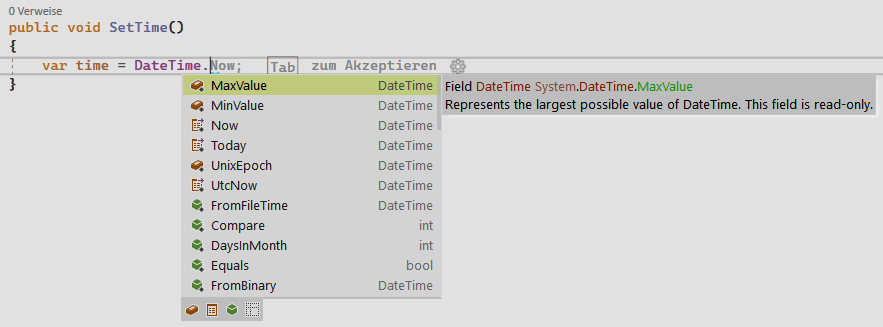
\includegraphics[width=125mm]{images/codecompletion.png}
	\caption{Code Vervollständigung in Visual Studio 2022}
	\label{fig:codecompletion}
\end{figure}
\FloatBarrier
Je mehr Zeichen bereits geschrieben wurden, desto genauer können die Vorschläge werden. Dies liegt daran, dass durch die schon geschriebenen Zeichen gewisse Optionen auszuschließen sind. Die Eingabe wird also ständig geparst und es ergeben sich mögliche Ergebnisse mit dem gleichen Präfix. Das Parsen kann beispielsweise durch reguläre Ausdrücke oder das Aufbauen von abstrakten Syntaxbäumen umgesetzt werden. Hierbei wird von der lexikalischen Analyse gesprochen. Ein anderer klassischer Ansatz ist die semantische Analyse. Diese verwendet ein Grammatikmodell der Sprache um anhand definierter Regeln nur Methoden anzuzeigen, welche auch legal sind. Dabei werden beispielsweise private Methoden herausgefiltert, wenn auf diese kein Zugriff vorhanden ist \cite{MarasoiuChurchBlackwell2015}. In der Regel werden beide Analysearten verwendet. 

Die Bestimmung der besten Ergebnisse ist dann durch verschiedene Implementierungen umsetzbar. Einfachste Lösung ist die Sortierung nach alphabetischer Reihenfolge oder dem Zeitpunkt der letzten Modifikation einer Methode. Auch denkbar ist die Priorisierung nach Lokalität, also beispielsweise zuerst die aktuelle Klasse, dann das Projekt und zuletzt Imports \cite{HobbesLanza2008}. 

Naheliegend ist auch die Sortierung nach der Anzahl der bisherigen Verwendungen eines Vorschlages. Diese Arten zählen zu den statistischen. Auch diese erzielen heutzutage bessere Ergebnisse, da öffentliche Repositories die notwendigen Daten zur Verfügung stellen. Anhand dieser können die Auftrittswahrscheinlichkeiten verschiedener Elemente ausgelesen werden um somit bessere Vorschläge zu erzielen. Verwendung findet dabei beispielsweise das N-Gram-Modell. Dieses zählt die Vorkommen verschiedener Kombinationen aus N Elementen \cite{Rosenfeld2000}. Problematisch ist, dass diese Modelle nur Abhängigkeiten zwischen wenigen Elementen feststellen. Außerdem funktioniert es nur, wenn Statistiken zu allen Element-Kombinationen vorhanden sind. 

Moderne Systeme nutzen immer häufiger einen anderen Ansatz: Künstliche Intelligenz. Im Gegensatz zur statistischen Analyse werden nicht nur Statistiken gesammelt sondern anhand von Daten wiederkehrende Muster erkannt. Diese schaffen es besser umfangreichen Kontext miteinzubeziehen und auf in den Trainingsdaten nicht vorhandene Elemente zu reagieren. Zur genauen Umsetzung gibt es verschiedenste Optionen. In \cite{Scharrenburg2019CodeCW} werden einige der verwendbaren rekurrenten neuronalen Netze gegenüber gestellt. Erwähnenswert ist außerdem der Algorithmus Best-Matching-Neighbour, welcher sich als sehr effizient herausgestellt hat \cite{BruchMonperrusMezini2009}.

\subsection{Nutzen und Risiken}
\label{subsec:completion_risks}
Die Nutzung von Codevervollständigung bringt zahlreiche Vorteile mit sich. Der größte ist die Zeitersparnis. Diese unterscheidet sich je nach Effektivität des Tools. Statt dem Ausschreiben ganzer Methodenaufrufe reicht oftmals der erste Buchstabe. Selbst wenn der gesuchte Vorschlag erst an dritter Stelle ist, muss nur zweimal die Pfeiltaste zur Auswahl betätigt werden. Im schlimmsten Fall müssen bereits mehrere Buchstaben vorhanden sein, damit die gesuchte Empfehlung kommt. Trotzdem findet eine enorme Zeiteinsparung statt. Gleiches gilt auch für die anderen Elemente, wie Variablen und Co. Einige Tools sprechen von ca. 40\% weniger Tastaturanschlägen \cite{Kite}. 
Außerdem werden durch die Vorschläge Tipp- und Logikfehler vermieden. Syntaktisch oder semantisch nicht korrekte Eingaben rufen keine Vorschläge hervor. Wird stattdessen die Eingabe durch Vorschläge vervollständigt, kann von syntaktischer und semantischer Korrektheit ausgegangen werden. Ein weiterer Vorteil ist, dass kein Detailwissen mehr benötigt wird. Sobald in objektorientierten Sprachen beispielsweise ein Punkt hinter das Objekt gesetzt wurde, werden dessen zugreifbare Methoden und Felder angezeigt. Dabei wird in der Regel bereits gefiltert, ob eine Zuweisung oder nur ein Aufruf stattfindet. Findet ersteres statt, werden nur Methoden und Felder mit Rückgabewert angezeigt. Besonders bei Nutzung fremder Bibliotheken ist dies von großem Vorteil. Somit können selbst schlecht dokumentierte Anwendungen und Bibliotheken verwendet werden, sofern die Namen verständlich gewählt wurden. Durch die Nutzung von Inline-Dokumentation sind die jeweiligen Methoden oftmals sogar direkt in der IDE beschrieben. 
Neben dem Vermeiden von Logik-Fehlern helfen diese Tools bereits beim Formulieren der Logik. Beispielsweise wird bei Zuweisung eines Wertes an eine Variable automatisch erkannt, wenn der Datentyp nicht übereinstimmt. Daher folgt ein Vorschlag zum Casting der Eingabe. Bei verschiedenen Collection-Arten werden dagegen beispielsweise auf diese anwendbare Strukturen wie \lstinline|foreach| vorgeschlagen. Das Gerüst dieser kann automatisch vervollständigt werden. Ein weiteres Beispiel ist die Rückgabe in einer Methode. Wird das passende Keyword geschrieben, kommen beispielsweise Vorschläge aus lokalen Variablen mit dem passenden Rückgabetyp. Die Beispiele sind zahlreich.

Diese Vorteile müssen allerdings mit Vorsicht genutzt werden. Die automatische Vervollständigung verleitet beispielsweise dazu, Vorschläge blind anzunehmen und einfach davon auszugehen, dass die dahinterliegende Funktionalität passend ist. Besonders bei fremden Bibliotheken wäre es dagegen sinnvoll, dies zu überprüfen oder die technische Dokumentation zu studieren. Gegebenenfalls hat eine verwendete Methode besonders schlechte Performance, ist bereits veraltet oder nicht Thread-safe, dies wird aber für die Anwendung benötigt. Hier muss zwingend vorsichtig vorgegangen werden.

\subsection{Marktanalyse}
\label{subsec:completion_analyse}
Es gibt verschiedene Tools zur Nutzung mit mehreren Sprachen. Bezüglich Microsoft und Visual Studio wird \textbf{IntelliSense} bzw. \textbf{IntelliCode} verwendet. Dieses unterstützt JavaScript, TypeScript, JSON, HTML, CSS, SCSS, C++, C\#, J\#, Visual Basic, XML, XSLT, SQL. Bei Nutzung der IDE Visual Studio Code ermöglichen Erweiterungen außerdem dutzende weitere Sprachen. Es basiert auf tausenden Repositories, deren Qualität durch eine Mindestanzahl an Sternen sichergestellt werden soll. 

Ähnlich viele Sprachen in verschiedenen Editoren unterstützt die alleinstehende Anwendung \textbf{Kite}. Diese wurden anhand von über 25 Millionen Dateien trainiert und soll die Tastenanschläge um ca. 40\% reduzieren \cite{Kite}. 

Besonders erwähnenswert ist allerdings das Projekt \textbf{Tabnine}. Es handelt sich um eine moderne, sehr umfangreiche Erweiterung. Bezüglich der Funktion Codevervollständigung ist diese kostenlos. Unterstützt werden 20 verschiedene IDEs und folgende Sprachen: Angular, C, C++, C\#, CSS, Dart, Go, Haskell, HTML, Java, Javascript, Kotlin, Matlab, NodeJS, ObjectiveC, Perl, PHP, Pyhton, React, Ruby, Rust, Sass, Scala, Swift und Typescript. Erkennbar ist das definierte Ziel, nicht auf spezielle Sprachen beschränkt zu sein. Besonderheit ist außerdem die Möglichkeit eigene Modelle zu trainieren indem ausgewählte Repositories verbunden werden. Dies ermöglicht die optimalen Vorschläge bezogen auf spezielle Projekte. So kann beispielsweise der Programmierstil innerhalb eines Unternehmens besser miteinbezogen werden. Dazu muss allerdings die kostenpflichtige Version (12€ pro User je Monat) in Verwendung sein. 
\begin{figure}[!htb] 
	\centering
	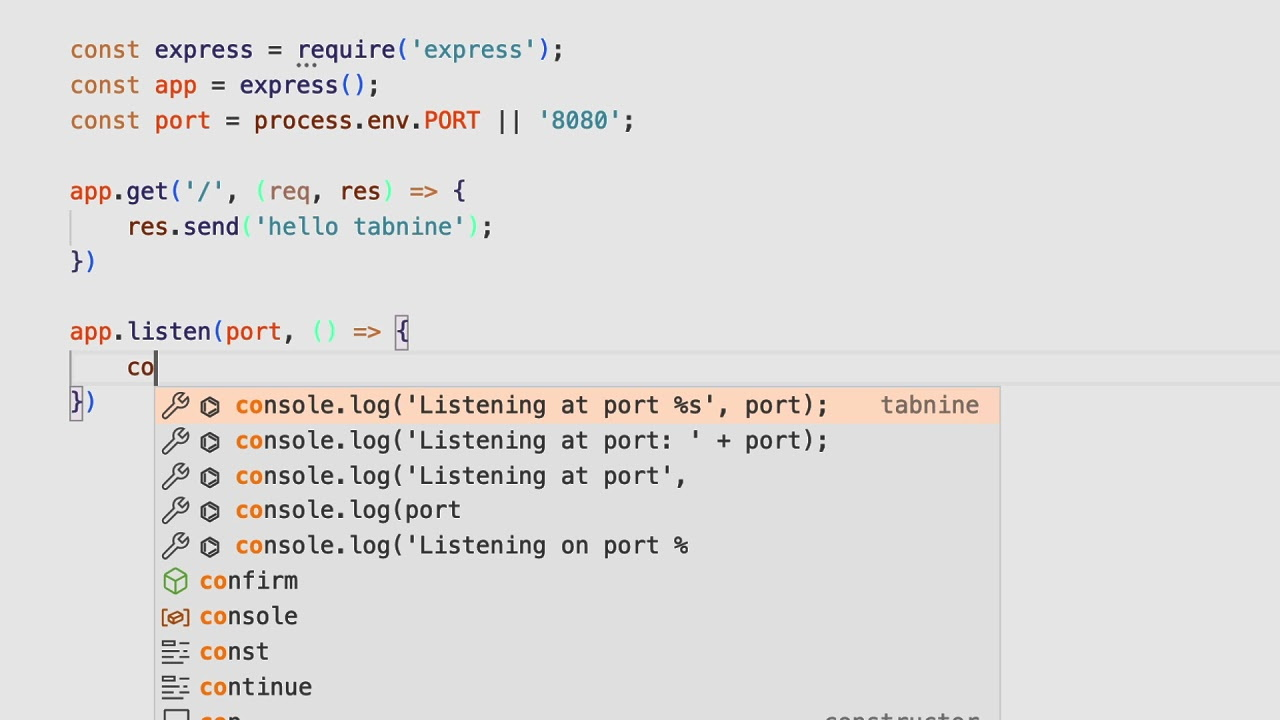
\includegraphics[width=125mm]{images/tabnine.jpg}
	\caption{Code Vervollständigung mit TabNine in VS Code}
	\label{fig:tabnine}
\end{figure}
\FloatBarrier
\autoref{fig:tabnine} zeigt die Vervollständigung durch TabNine in Visual Studio Code. Erkennbar ist, dass mehr als nur ein Methodenname vervollständigt wird. Anhand des Befehls \lstinline|app.listen(port, ...)| schlägt die Software einen passenden Text für das Logging unter Einbezug der Parameter vor. Als Grundlage von \textit{Tabnine} gilt das Modell GPT-2. Die verwendeten Daten stammen von GitHub-Repositories, für welche Qualität sichergestellt wurde. Neue Daten finden regelmäßig Einsatz im Training, um auch neuste Entwicklungen miteinzubeziehen.
\section{Codegenerierung}
\label{sec:codegeneration}
In bestimmten Fällen ist es mittlerweile nicht mehr notwendig Quellcode von Hand zu schreiben. Stattdessen kann spezifiziert werden, was der Programmcode tun soll und aus dieser Information automatisch Code generiert werden. Dieser Anwendungsfall kann zwar nicht so weitläufig eingesetzt werden wie die Codevervollständigung, spart stellenweise aber noch mehr Arbeit ein.

\subsection{Allgemeine Konzepte}
\label{subsec:generation_concepts}
Programmiersprachen dienen dazu Datenstrukturen und Algorithmen formal aber vom Menschen lesbar auszudrücken. Hierbei unterscheidet man zwischen High-Level- und Low-Level Programmiersprachen (\autoref{fig:abstractionLevels}). Low-Level Programmiersprachen befinden sich auf einer niedrigen, High-Level Programmiersprachen auf einer höheren Abstraktionsebene. Ziel dieser Abstraktion ist es, die Lesbarkeit zu erhöhen und die Komplexität zu reduzieren. Hierfür bieten High-Level Programmiersprachen beispielsweise Kontrollstrukturen und Datentypen an.
Bei der Codegenerierung wird diese Idee aufgegriffen und erweitert.
Im Allgemeinen geht es um die Frage, ob es nicht einfachere und kompaktere Darstellungsweisen für Problemlösungen gibt, die anschließend in Programmcode einer tieferen Abstraktionsebene umgewandelt werden können. 
\begin{figure}[!htb] 
	\centering
	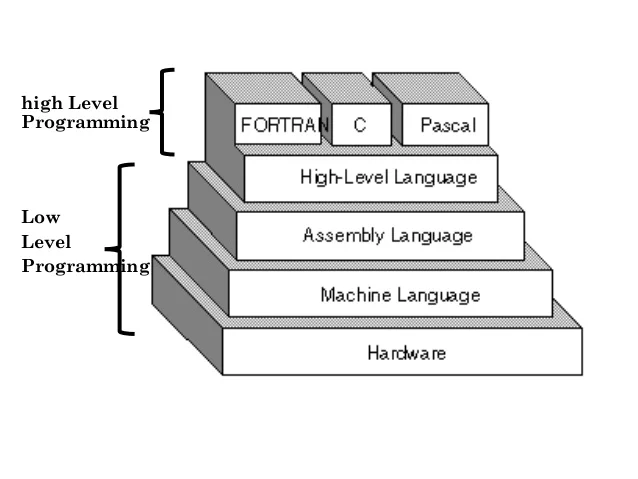
\includegraphics[width=12cm]{images/abstractionlevel_programminglangs.png}
	\caption{Abstraktionsebenen von Programmiersprachen \cite{abstractionlevels_img}}
	\label{fig:abstractionLevels}
\end{figure}
\FloatBarrier

Ein \textbf{Compiler} ist wohl das bekannteste Werkzeug zur Codegenerierung. Dieser wandelt Quellcode einer höheren Programmiersprache in Befehle einer niedrigeren Sprache um.
Ein Compiler für die Programmiersprache Java besteht aus verschiedenen Bestandteilen: Ein Scanner liest Lexeme und generiert Tokens. Der Parser generiert eine abstrakte Syntax. Im Semantik-Check wird eine getypte abstrakte Syntax generiert. Zuletzt generiert ein Code-Generator Bytecode für die JVM. Compiler sind ein fester Bestandteil von nahezu jedem Softwareentwicklungsprozess und werden aus diesem Grund der Vollständigkeit halber hier angemerkt, jedoch nicht näher behandelt.

\textbf{Modellgetriebene Softwareentwicklung (MDSD)} \textit{ist ein Oberbegriff für Techniken, die aus formalen Modellen automatisiert lauffähige Software erzeugen.} \cite[p.~11]{StahlVoelterEtAl07}

Die formalen Modelle werden meist im zugeschnittenen Modellierungssprachen wie DLS oder UML spezifiziert. Formal bedeutet in diesem Zusammenhang, dass das Modell einen bestimmten Aspekt der Software vollständig beschreibt. Dies ist essentiell für die anschließend automatische Codeerzeugung.
Ein wichtiger Begriff in diesem Kontext ist das Round-Trip Engineering. Dies beschreibt die bidirektionale Synchronisation zwischen Modellen und Quellcode. So können die Vorteile der Modellentwicklung (Übersichtlichkeit und Dokumentation) mit den der Quellcodeprogrammierung (Präzision und Spezifikation) kombiniert werden.

Die Vorteile einer modellgetriebenen Softwareentwicklung sind \cite[p.~13-16]{StahlVoelterEtAl07}:
\begin{itemize}
	\item[(a)] \textbf{Abstraktion:} Die Modelle sind einfacher und allgemeiner als der zu generierende Quellcode.
	\item[(b)] \textbf{Einheitliche Architektur:} Die Softwareerzeugung aus den Modellen erfolgt nach streng formalen Vorschriften unter Berücksichtigung eines vorgegebenen Rahmens. 
	\item[(c)] \textbf{Softwarequalität}
	Das Projekt wird durch den modellgetriebenen Entwicklungsprozess in eine einheitliche, testbare und dokumentierte Architektur gegossen. Selbstverständlich ist dies dennoch keine Garantie für gute Softwarequalität.
	\item[(d)] \textbf{Entwicklungsgeschwindigkeit:}  Durch eine höhere Softwarequalität ist das Projekt besser Wartbar und Komponenten sind besser Austauschbar, was langfristig die Entwicklungsgeschwindigkeit erhöht. Zudem gibt es immer eine Designdokumentation, was die Übersichtlichkeit erhöht.
	\item[(e)] \textbf{Interoperabilität und Plattformunabhängigkeit:} Durch die modellgetriebene Entwicklung soll eine Plattform- und Frameworkunabhängigkeit durch Standardisierung erreicht werden. Die Modelle sollen streng vom generierten Programmcode entkoppelt und somit von diesem unabhängig sein. Dies ist jedoch meist nur in der Theorie möglich und kann beispielsweise beim Round-Trip Engineering nicht gewährleistet werden.
\end{itemize}

Die Nachteile der modellgetriebenen Entwicklung sind:
\begin{itemize}
	\item[(a)] \textbf{Hoher Initialisierungsaufwand:}
	Der Initialisierungsaufwand ist sehr hoch und zahlt sich entsprechend nur bei großen Projekten aus.
	\item[(b)] \textbf{Hoher Einarbeitungsaufwand:}
	Da die modellgetriebene Entwicklung nicht so verbreitet ist wie die Verwendung herkömmlicher Programmiersprachen, jedoch eine hohe Komplexität aufweist, ist ein hoher Einarbeitungsaufwand notwendig.
\end{itemize}

Werkzeuge für die modellgetriebene Entwicklung fangen bei einfachen UML-Codegeneratoren (z.B. Visual Paradigm) an und hören bei Komplettlösungen für bestimmte Domänen (z.B. ASCET für eingebettete Automobilsoftware) auf \cite{StahlVoelterEtAl07}.

Durch AI-basierte Werkzeuge gibt es die Möglichkeit zur \textbf{Quellcodeerzeugung aus natürlicher Sprache}. Dies stellt sich vor allem für stark spezialisierte Bereiche als nützlich heraus. Ein Beispiel hierfür ist die Generierung von SQL Statements oder einfachen Programmieranweisungen aus natürlicher Sprache. 

Eine populäre Möglichkeit hierfür ist das AI-Modell OpenAI Codex. Dieses stellt auch die Basis für das Werkzeug GitHub Copilot dar, welches gemeinsam von OpenAI und GitHub entwickelt wurde \cite{openaicodex}.
Dieses Modell kann über die API oder dem Browser-Playground von OpenAI genutzt werden.
In einem Test wurde ein Ratespiel in JavaScript mittels dem OpenAI Codex Model generiert (\autoref{code:naturallangcodegen}). Aus dem in den Kommentaren angegebene Text in natürlicher Sprache wurde jeweils der darunter stehende Quellcode generiert.
\begin{lstlisting}[caption={Code aus natürlicher Sprache}, label=code:naturallangcodegen]

/* Generiere eine zufaellige Zahl zwischen 0 und 10 */
var randomNumber = Math.floor(Math.random() * 10);

/* Frage den Nutzer nach einer Texteingabe */
var userInput = prompt('Gib eine Zahl zwischen 0 und 10 ein');

/* konvertiere die Nutzereingabe in eine Zahl */
var userNumber = parseInt(userInput);

/* wenn die generierte Zufallszahl gleich der userNumber ist "gewonnen", sonst "verloren" ausgeben */
if (randomNumber === userNumber) {
	alert('gewonnen');
} else {
	alert('verloren');
}
\end{lstlisting}
\FloatBarrier
Auch die Generierung von SQL Statements liefert ein korrektes Ergebnis (\autoref{code:naturallangsql}).
\begin{lstlisting}[caption={SQL Statement aus natürlicher Sprache}, label=code:naturallangsql]
### Postgres SQL tables, with their properties:
#
# Mitarbeiter(mid, vorname, nachname)
# Teilnahme(mid, pid)
# Projekt(pid, bezeichnung)
#
### Liste die Mitarbeiternamen der Mitarbeiter des Projektes "Test" auf
---------------------------------------------------------------------
SELECT m.vorname, m.nachname
FROM Mitarbeiter m
JOIN Teilnahme t ON m.mid=t.mid
JOIN Projekt p ON t.pid=p.pid
WHERE p.bezeichnung='Test'
\end{lstlisting}
\FloatBarrier
Selbst etwas komplexere Aufgaben, wie API-Aufrufe und Deserialisierung sind möglich. Hierzu musste jedoch mit der textuellen Eingabe etwas experimentiert werden (\autoref{code:naturallangapi}) \cite{openaicodexsandbox}.
\begin{lstlisting}[caption={API Aufruf und Deserialisierung aus natürlicher Sprache}, label=code:naturallangapi]
//API aufrufen: https://jsonplaceholder.typicode.com/todos/1 
//Ergebnisse Deserialisieren & Ausgeben
//Quellcode in C#:
-------------------------------------------------------------------
using System;
using System.IO;
using System.Net;
using System.Runtime.Serialization.Json;

namespace ConsoleApp1
{
	class Program
	{
		static void Main(string[] args)
		{
			string url = @"https://jsonplaceholder.typicode.com/todos/1";
			WebRequest req = WebRequest.Create(url);
			req.Method = "GET";
			WebResponse resp = req.GetResponse();
			var json = new DataContractJsonSerializer(typeof(Todo));
			var todo = (Todo)json.ReadObject(resp.GetResponseStream());
			Console.WriteLine(todo);
		}
	}
	
	[DataContract]
	public class Todo
	{
		[DataMember]
		public bool completed { get; set; }
		[DataMember]
		public int userId { get; set; }
		[DataMember]
		public int id { get; set; }
		[DataMember]
		public string title { get; set; }
		
		public override string ToString()
		{
			return $"{completed} {id} {title}";
		}
	}
}
*/
\end{lstlisting}
\FloatBarrier
Nüchtern betrachtet bieten solche Modelle dem Entwickler jedoch kaum eine Zeitersparnis und die Ergebnisse müssten zudem stets manuell auf Korrektheit überprüft werden. Als unterstützendes Werkzeug können solche Modelle jedoch nützlich sein. Wenn der Entwickler beispielsweise nicht mit einer Programmiersprache vertraut ist, können Befehle (wie z.B. die Ein- und Ausgabe) mittels natürlicher Sprache umschrieben werden. Für die Erstellung komplexer Software sind solche Generierungsverfahren jedoch ungeeignet, da die Umschreibung mit natürlicher Sprache meist zu unscharf und inkonsistent ist \cite{DBLP:journals/corr/abs-2107-03374}. 

\textbf{Weitere Möglichkeiten}, die jedoch nur gewisse Spezialgebiete der Softwareentwicklung abdecken sind folgende \cite{Dollard2008}: Annotationen, Präprozessoranweisungen, O/R-Mapper, Interface-Definition-Languages oder Codeerzeugung durch grafischen Oberflächendesigner.

%Moderne objektorientierte Programmiersprachen wie Java und C\# bieten die %Möglichkeit Quellcode zu annotieren. Annotationen können zum einen über %Reflection zur Laufzeit ausgewertet werden und hierdurch ein bestimmtes %implementiertes Verhalten bewirken. Zum anderen gibt es bestimmte %Annotationen, die vom Compiler ausgewertet und verarbeitet werden.
\subsection{Vorteile und Grenzen}
Codegenerierung kann in der Softwareentwicklung unterschiedlich eingesetzt werden und bestimmte Vorgänge erleichtern (wie bereits in den Unterabschnitten beschrieben). Während die modellgetriebene Softwareentwicklung ein gesamtes Paradigma darstellt, sind Werkzeuge wie OpenAI Codex nur für bestimmte Randgebiete sinnvoll. Unabhängig vom verwendeten Codegenerator gilt weiterhin das bekannte Garbage In, Garbage Out Prinzip der Informatik. Darüber hinaus muss für jeden Anwendungsfall abgeschätzt werden, ob das verwendete Werkzeug einen Zeit, Qualitäts oder Produktivitätsgewinn darstellt oder eher hinderlich ist. Zu erwähnen ist außerdem, dass diese Entwicklung noch lange nicht abgeschlossen ist. Es bleibt abzuwarten was bessere Modelle und immer mehr Beispieldatensätze in Zukunft ermöglichen werden.

\section{Analyse}
\label{sec:codeanalyse}
Wurden Teile eines Programms programmiert, ist es wichtig dessen Funktion und Leistung zu überprüfen. Neben der Identifikation von Problemen geht es dabei vor allem um Optimierungen. Dieser Abschnitt beschäftigt sich mit automatisierten Verfahren zur Analyse von Software. Zunächst werden die allgemeinen Konzepte statische und dynamische Analyse erklärt. Darauffolgend werden die Vorteile und Grenzen dieser Verfahren erläutert. Abschließend wird ein Werkzeug zur Analyse von Software vorgestellt. 

\subsection{Allgemeine Konzepte}
Die \textbf{statische Quellcodeanalyse} ist ein Verfahren, welches Quellcode unabhängig von der Kompilierung oder Ausführung nach verschiedenen Kriterien auswertet. Dies soll Fehler, Inkonsistenzen und Unsicherheiten im Programmcode aufdecken. Statisch bedeutet in diesem Kontext, dass der Code nicht ausgeführt, jedoch unter anderem auch semantisch ausgewertet wird. Verwendete Verfahren sind \cite[p.~12]{OwaspCodeReview2008}:
\begin{itemize}
	\item[(a)] \textbf {Taint Analyse}: Analyse zur Verhinderung von böswilligen Benutzereingaben, die Code auf dem Hostcomputer ausführen (z.B. SQL Injection)
	\item[(b)] \textbf {Datenfluss Analyse}: Analyse, welche Daten zwischen Programmteilen ausgetauscht werden und welche Abhänigkeiten daraus entstehen.
	\item[(c)] \textbf {Kontrollfluss Analyse}: Analyse zur Evaluation und Integritätsprüfung des Programmablaufes mit dem Ziel der Feststellung von Anomalien (z.B. Endlosschleifen)
	\item[(d)] \textbf {Lexikalische Analyse}: Syntaktische Prüfung des Quellcodes und Generierung von Tokens
\end{itemize}
Historisch ist das Programmierwerkzeug Lint der Pionier der statischen Codeanalyse. Ursprünglich wurde Lint für die Programmiersprache C entwickelt. Nach und nach wurden Abwandlungen für andere Programmiersprachen, darunter beispielsweise JavaScript, TypeScript und Python, entwickelt. Die Entwicklung von Lint lief synergetisch zu der Entwicklung moderner Compiler \cite[p.~2] {Darwin1988}. Ursprünglich sind Lint Programme so gedacht, dass diese vom Benutzer explizit ausgeführt werden müssen und anschließend den Quellcode analysieren.
In modernen IDE sind Lint-ähnliche Verfahren meist automatisch integriert. Diese analysieren kontinuierlich den Quellcode und zeigen mögliche Probleme direkt an (\autoref{fig:lint_vs}). 
Zudem werden solche Analysewerkzeuge als zusätzliche Plugins für viele IDEs angeboten \cite{Darwin1988}\cite{wiki:Lint_Programmierwerkzeug}.

\begin{figure}[!htb] 
	\centering
	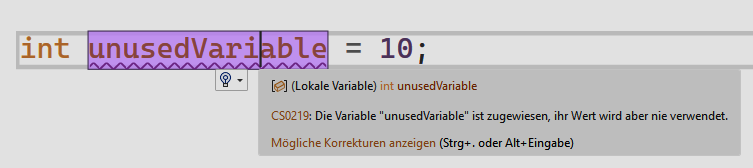
\includegraphics[width=125mm]{images/ide_linting.png}
	\caption{Statische Codeanalyse in Visual Studio}
	\label{fig:lint_vs}
\end{figure}
\FloatBarrier

Die Möglichkeiten der statischen Codeanalyse lassen sich in die Kategorien \textit{Stylechecking}, \textit{Semantische Analyse} und \textit{Weiteres} unterteilen.

\label{subsubsec:style}Bei der Softwareentwicklung wird häufig im voraus ein Programmierstil, auch oft Coding Conventions genannt, festgelegt. Dieser baut auf den üblichen Vorgehensweisen des verwendeten Programmierparadigma auf. Die meisten Programmiersprachen bieten ein Katalog von solchen Codierungsrichtlinien an. So existiert beispielsweise für die objektorientierte Sprache Java ein Dokument mit einer Empfehlung für einen zu verwendenden Programmierstil \cite{java_coding_conventions}.

Für Projekte ist es gegebenenfalls sinnvoll die Codierungsrichtlinien der verwendeten Programmiersprache anzupassen und zu erweitern.
Beispiele für Codierungsrichtlinien sind die Anwendung von Entwurfsmustern, die Festlegung der Namenskonventionen, der Umfang der Dokumentation oder die Gestaltung von Funktionsaufrufen.

Ein \textbf{Style Checker} ist ein Werkzeug, welches die Einhaltung des definierten Programmierstils überprüft. Dies ermöglicht es beispielsweise Verstöße gegen Benennungskonventionen oder einer Überschreitung der maximal zulässigen Zeilenlänge von Code zu erkennen. Style Checker bilden jedoch nur eine Teilmenge davon ab, was mit statischer Codeanalyse möglich ist, da meistens keine semantische Quellcodeanalyse vorgenommen wird.  So kann beispielsweise nicht erklärt werden, dass in \autoref{code:infiniteloop} eine Endlosschleife produziert wurde \cite{lwn.net}\cite{wiki:Style_Checker}.
\begin{lstlisting}[caption={Endlosschleife}, label=code:infiniteloop]
	while (1<10)
	{
	}
\end{lstlisting}
\FloatBarrier
In der \textbf{semantischen Analyse} wird der Quellcode auf inhaltliche Konsistenz und mögliche Fehler geprüft. So können beispielsweise folgende Probleme erkannt werden: Memory Leaks, Pufferüberläufe, Divisionen durch null, Array Zugriffe außerhalb der Grenzen, Endlosschleifen, mögliche Nullverweise, nicht verwendete Variablen und Methoden, Anti-Patterns, mögliche Code Injections, Substitutionen und Generalisierungen oder toter Quellcode. Diese Art der Analyse ist besonders wichtig, da sie folgenschwere Fehler aufdecken soll.

Wird ein objektorientiertes Programmierparadigma verwendet besteht eine \textbf{weitere Möglichkeit} in der Bestrebung durch statische Quellcodeanalysen das Design zu bewerten. Dies ist natürlich nicht vollumfänglich möglich, jedoch gibt es bestimmte statisch ermittelbare Metriken, die 
auf ein gutes oder schlechtes Design schließen lassen. Diese lassen sich aus den Prinzipien für ein agiles, objektorientiertes Design ableiten \cite{Martin2002-nf}. Folgende Metricken sind hierfür denkbar und teilweise auch schon in statischen Analysewerkzeugen implementiert \cite{OwaspCodeReview2008}\cite{Darwin1988}\cite{jetbrains_static_analyse}\cite{wiki:Statische_Code-Analyse}:
\begin{itemize}
	\item[(a)] Lines of Code (Single Responsiblility)
	\begin{itemize}
		\item Innerhalb einer Komponente, Komponente oder Methode
	\end{itemize}	
	\item[(b)] Ringabhänigkeiten
	\item[(c)] Coderedundanzen (Don't repeat yourself, Abstraction)
	\item[(d)] Große Vererbungsstrukturen (Composition over inheritance)
	\item[(e)] Abhänigkeiten auf Implementierungen statt auf Interfaces (Dependency Inversion, Open-Closed)
	\item[(f)] Größe der Interfaces (Interface Seggregation)
	\item[(g)] Fehlende Implementierungen für Basismethoden (Liskov Subsitution)
\end{itemize}

Bei der \textbf{dynamischen Analyse} liegt der Fokus auf Bereichen, die nicht von der statischen Quellcodeanalyse abgedeckt werden können. Dies sind primär Fehler in der Anwendungslogik, fehlende Sicherheitsvalidierung und Performance. 

Wesentlich wird die dynamische Analyse von sogenannten Profiling Werkzeugen abgewickelt. Diese können verschiedene Messwerte zu der entwickelten Software ermitteln. Dazu gehört die Anzahl der Funktionsaufrufe und Funktionsdurchläufe, die Speicherauslastung, nicht freigegebenen Speicherbereiche, nebenläufige Prozesse und Deadlocks. Durch statistische Analysen kann herausgefunden werden, welche Programmteile lohnenswert optimierbar sind, um eine bessere Leistungs- und Speicherperformance zu erhalten. Auch Fehler in der Anwendungslogik, die sich in Deadlocks oder Memoryleaks manifestieren, können aufgedeckt werden \cite{mci/Papenbrock2019}\cite{wiki:Profiler_Programmierung}\cite{computerweekly_dynamic_code}\cite{embedded_swe_codeanalysis}. \label{subsubsec:dynamic}


\subsection{Vorteile und Grenzen}
\label{subsec:Codeanalyse_risks}
Durch Automatisierte Analyseverfahren können tausende Zeilen Quellcode in kürzester Zeit mit einer sehr hohen Präzision durchsucht und ausgewertet werden. Mögliche Problemstellen werden unmittelbar angezeigt und können meist auch zur Quelle zurückverfolgt werden (z.B. nicht validierte Parameter). Über Konfigurationen können die Codeconventions festgelegt werden und Antipatterns definiert werden, die anschließend bei der statischen Codeanalyse überprüft werden. So kann auch in großen Projekten eine Einheitlichkeit und Stabilität im Quellcode erreicht und somit die Softwarequalität erhöht werden.
Häufig auftretende Probleme oder Muster, die zu Schwierigkeiten im Entwicklungsprozess führen können, sind in den Analysewerkzeugen bereits vorkonfiguriert.
Intellegente Analysewerkzeuge bieten zudem die Möglichkeit einer automatischen Problembehebung. Hier wird der Quellcode automatisch refaktorisiert (\autoref{sec:refactor}) oder abgeändert.

Auch wenn Analysewerkzeuge eine große Hilfe für Softwareentwickler darstellen, ist es wichtig die Grenzen dieser zu kennen. Analysewerkzeuge sind nur so gut, wie sie programmiert und konfiguriert wurden. Sind bestimmte Antipatterns oder Konstrukte für unsauberen Code nicht in der Konfiguration und Programmierung berücksichtigt, werden diese auch nicht erkannt. Zudem lassen sich auch technisch nicht alle Problemfelder ermitteln. So können Logikfehler in komplexen Geschäftsprozessen häufig nicht identifiziert werden, da das Analysewerkzeug kein Verständnis hierfür besitzt. Auch bei Framework-spezifischen Anwendungsfeldern können Probleme auftreten, da die Analysewerkzeuge auf die Framework Version abgestimmt sein müssen. Werden spezielle Techniken verwendet, wie z.B. Dependency Injection, die bei der Implementierung des Werkzeuges nicht berücksichtigt sind, kann es ebenfalls zu Schwierigkeiten kommen. So kann es in diesem Fall sein, dass Abhängigkeiten nicht mehr nachvollzogen werden können, weil keine klassische Referenzerzeugung und Übergabe mehr stattfindet. Sprachen die ständig weiter entwickelt werden, erzwingen ebenfalls eine kontinuierliche Weiterentwicklung der zugehörigen Analysewerkzeuge \cite{OwaspCodeReview2008}\cite{wiki:Statische_Code-Analyse}\cite{embedded_swe_codeanalysis}. 

\subsection{Beispiel Werkzeug}
\label{subsec:Codeanalyse_analyse}
Als eine Suite von Beispielwerkzeugen werden die Produkte des Softwareherstellers JetBrains gewählt. Die Werkzeuge sind entweder in die IDEs, die von Jetbrains angeboten werden integriert, oder als seperates Plugin für Visual Studio oder den Standalonebetrieb verfügbar. Angeboten werden:
\begin{itemize}
	\item[(a)] ReSharper (Statische Codeanalyse, Refactoring)
	\item[(b)] DotTrace (Dynamische Analyse, Leistungsprofiling)
	\item[(c)] DotMemory (Dynamische Analyse, Memoryprofiling)
	\item[(d)] DotCover (Statische und dynamische Analyse, Testabdeckung, Unittesting)
\end{itemize}
Jetbrains bietet elf IDEs für verschiedene Programmiersprachen an, die alle auf einem gemeinsamen Framework basieren \cite{intelliJPlattform}. Somit werden die Sprachen Objective C, Swift, PHP, Python, C\#, Visual Basic, Go, Rust, Ruby, Kotlin, JavaScript und Java unterstützt \cite{jetbrains_products}. 
%https://faculty.sist.shanghaitech.edu.cn/faculty/songfu/cav/PPA.pdf
%Artificial Intelligence Methods For Software Engineerin
%https://de.wikipedia.org/wiki/Statische_Code-Analyse
%https://www.techtarget.com/searchsoftwarequality/news/252523049/Developers-beware-AI-pair-programming-comes-with-pitfalls
%https://dl.acm.org/doi/pdf/10.1145/318774.318944
%file:///D:/Users/Jona/Downloads/ESSCAT-report-for-printing-1.pdf
\section{Refactoring}
\label{sec:refactor}
Nach einer Analyse stehen in der Regel Änderungen im Code an. \textit{Refactoring}, oder zu Deutsch \textit{Refaktorierung}, beschreibt die nachträgliche Veränderung von Quellcode in Software. Konkret wird unter Beibehaltung des Verhaltens eines Programms eine verbesserte Struktur erzielt. Es ist also abgegrenzt von der Entwicklung neuer Funktionalitäten. Dies sollte vor allem bei großen Projekten ständiger Bestandteil sein. Schlechter Code erzeugt sonst immer größere Probleme und senkt somit auf Dauer die Produktivität \cite[S. 28]{martin2009}. Stattdessen sollte sauberer Code angestrebt werden. Dies bezieht sich sowohl auf Softwarearchitektur, als auch generelle Lesbarkeit von Code. Clean Code wird zum einen durch die im vorherigen Kapitel (\autoref{sec:codeanalyse}) genannten Kriterien, oder auch die ISO-Normen, auf höherer Ebene analysiert. Eine Sicht auf niedrigerer Ebene bietet Grady Booch, Autor von \textit{Object-Oriented Analysis and Design with Application}:
\begin{center}
	\textit{Sauberer Code ist einfach und direkt. Sauberer Code liest sich wie wohlgeschriebene Prosa. Sauberer Code verdunkelt niemals die Absicht des Designers, sondern ist voller griffiger (engl. crisp) Abstraktionen und geradliniger Kontrollstrukturen.} \cite[S. 34]{martin2009}
\end{center}
Durchgehend sauberer Code ist zum Beispiel aufgrund von sich verändernden Anforderungen schwer zu erreichen. Daher ist Refactoring ein derart wichtiger Prozess. Da Refactoring aber auch bedeutet, dass in dieser Zeit keine neuen Funktionen entwickelt werden, ist die Balance sehr wichtig.

\subsection{Betroffene Stellen}
\label{subsec:whereRefact}
Betroffen sind zum Einen die Ergebnisse von Analysen, welche Probleme aufgezeigt haben. Diese wurde im vorherigen Kapitel (siehe \autoref{sec:codeanalyse} erläutert). Weitere unsaubere Stellen im Code werden auch "Code-Smell" genannt \cite[S. 67]{fowler2000}. Martin Fowler kategorisiert diese in 22 Arten der Probleme \cite[S. 67 - S. 82]{fowler2000}. Diese können teilweise in der Analyse erkannt werden, erfordern aber oftmals auch manuelle Überprüfung. Im Folgenden sind die wichtigsten zusammengefasst und erklärt:
\begin{itemize}
	\item[(i)] \textbf{Redundanter Code} verringert die Änderbarkeit, sorgt für doppelte Entwicklung und großen Overhead.
	\item[(ii)] \textbf{Große Methoden, Parameterlisten oder Klassen} sind schwer verständlich und weniger Wiederverwendbar. Weitere mögliche Probleme sind schlechte Testbarkeit und Verletzung des Single Responsibility Prinzips.
	\item[(iii)] \textbf{Hinzufügen von nicht zugehörigen Funktionalitäten zu einer Klasse} verletzt das \textit{Single Repsonsibilty}-Prinzip und verschlechtert somit die Wartbarkeit. Gleiches gilt für das Gegenteil, also die Aufteilung einer Funktionalität auf verschiedene Klassen. Jede Klasse sollte also eine Verantwortlichkeit haben.
	\item[(iv)] \textbf{Unübersichtliche Gruppen aus zusammengehörigen Parametern anstelle der Nutzung eines Objektes} schaden der Lesbarkeit und sorgen für geringere Wartbarkeit. Änderungen müssen immer an allen Stellen, statt nur in der definierten Klasse erfolgen.
	\item[(v)] \textbf{Verschachtelte Switch-Befehle} behindern die Lesbarkeit. Je mehr Ebenen im Code sind, desto unübersichtlicher wird es.
	\item[(vi)] \textbf{Nachrichtenketten} schaden der Performance durch zu viele Zwischenaufrufe.
	\item[(vii)] \textbf{Klassen ohne eigene, nicht-triviale Verantwortlichkeit} schaden der Wartbarkeit und deuten auf schlechte Architektur hin.
	\item[(viii)] \textbf{Unangebrachte Abhängigkeiten von Details statt Schnittstellen} sorgen für schlechte Austauschbarkeit. Gleiches gilt für funktional gleiche Klassen, welche unterschiedliche Schnittstellen anstelle einer gemeinsamen besitzen.
	\item[(ix)] \textbf{Übermäßige Kommentare} implizieren eine Unverständlichkeit des Codes und schaden der Lesbarkeit.
	\item[(x)] \textbf{Nichtssagende Namen} sorgen für schlechte Lesbarkeit und Problemen bei späteren Änderungen.
\end{itemize}
Es könnten viele weitere genannt werden, genauere Details bietet auch Robert Martin in seinem Buch \textit{Clean Code} \cite{martin2009}.

\subsection{Allgemeine Konzepte zur Lösung}
\label{subsec:Refactoring_concepts}
In seinem Buch \textit{Refactoring} stellt Martin Fowler einen großen Katalog von möglichen Refactorings auf \cite[S. 99 - 387]{fowler2000}. Im Folgenden findet eine Betrachtung einiger ausgewählter Refactorings statt, welche automatisch von Software umgesetzt werden können. Viele weitere sind manuell durchführbar, aber nicht Teil dieser Arbeit. 
\begin{itemize}
	\item[(a)] \textbf{Extrahieren oder Verschieben von Methoden und Klassen}: Ist eine Methode zu lange (siehe i), kann ein Teil von ihr ausgewählt und in eine eigene Methode extrahiert werden. Die Software erkennt Rückgabewert und Parameter automatisch, nur der Methodenname muss gewählt werden. Problematisch zur Auslagerung können dabei die lokalen Variablen sein. Diese müssen oftmals von Hand angepasst werden, zum Beispiel durch die Aufteilung in kleinere Variablen.
	Klassen dagegen werden oftmals in einer anderen Klassendatei definiert. Software ermöglicht das Verschieben in eine eigene Datei, was der Übersichtlichkeit dient. 
	\item[(b)] \textbf{Vereinfachen von Ausdrücken und Statements}: Aufgrund vorheriger Analysen wurden mögliche Vereinfachungen im Code erkannt (\autoref{subsec:Codeanalyse_analyse}). Die Software macht daraufhin Vorschläge zur Umwandlung. Dies kann beispielsweise die Invertierung einer If-Abfrage sein, welche für höhere Übersichtlichkeit sorgt. Oder auch die Umwandlung einer Verkettung von If-Abfragen in ein Switch-Statement. Ein anderes Beispiel wäre die Vereinfachung eines bedingten Ausdruckes, da die gleiche Logik in kompakterer Form erreicht werden kann.
	\item[(c)] \textbf{Umbenennung von Bezeichnern}: Aussagekräftige Bezeichner sind besonders wichtig (siehe x), da Quellcode sich selbst erklären soll. Software ermöglicht das Umbenennen eines Bezeichners an all seinen Vorkommen. Dies erspart Arbeit und die Gefahr, nicht alle Verwendungen zu finden. Oftmals weißt ein Stylechecker (\autoref{subsubsec:style}) auf problematische Bezeichner hin und bietet Gegenvorschläge.
	\item[(d)] \textbf{Migration von Datentypen}: Wird einer Variable oder einem Feld ein falscher Typ zugewiesen, muss dieser migriert bzw. geparst oder der Datentyp des Felder verändert werden. Software kann diese Lösungen automatisch vornehmen.
	\item[(e)] \textbf{Einführung von Feldern oder Variablen}: Oftmals findet eine hohe Verschachtlung statt, was ein Zeichen für Code-Smell ist (siehe v). In der Regel ist eine Extraktion in erklärende Variablen sinnvoll. Dies kann durch Software erledigt werden, nur die Auswahl des Namens muss stattfinden.
	\item[(f)] \textbf{Parameter ergänzen, entfernen oder überladen}: Wird eine Methode aufgerufen mit anderen Parametertypen, als aktuell definiert, gibt es verschiedene Möglichkeiten. Entweder wird die Parameterliste verändert oder es muss eine Überladung der Methode mit passenden Parametern erzeugt werden. Dies kann eine Software automatisch übernehmen.
	\item[(g)] \textbf{Schnittstelle implementieren}: Implementiert eine Klasse ein Interface, muss es alle dessen Methoden überschreiben. Software ermöglicht das Einfügen aller Methoden des Interfaces mit leerem Methodenkörper. 
	\item[(h)] \textbf{Attribute kapseln}: Ein Kernprinzip der objektorientierten Programmierung ist die Datenkapselung über Getter und Setter. Diese können ausgehend von einem Feld automatisch erzeugt werden durch Software.
	\item[(i)] \textbf{Maximale Abstraktion verwenden}: Sofern es möglich ist, sollte immer maximale Abstraktion und minimales Detail verwendet werden (siehe viii). Wird daher in der Analyse erkannt, dass eine höhere Abstraktion verwendbar ist, kann der Objekttyp automatisch ausgetauscht werden.
	\item[(j)] \textbf{Verwenden und Austausch von Modifzierern}: Verschiedene Modifizierer für Variablen können Vorteile bieten, so beispielsweise wenn ein String als Konstante definiert wird. Wurde in der Analyse erkannt, dass dies möglich ist, kann der Modifizierer durch die Software automatisch eingefügt werden. Gleiches gilt bezüglich Sichtbarkeit. Ist eine höhere Kapselung möglich, also beispielsweise protected statt public, kann die Änderung automatisch vollzogen werden.
	\item[(k)] \textbf{Formatierung}: Neben Architektur und Benennungen ist vor allem die Formatierung des Codes ausschlaggebend für Übersichtlichkeit. Software bietet hier die Möglichkeit, diese nach einem definierten Schema vorzunehmen. Es handelt sich um ein sogenanntes \textit{Beautify} des Codes.
	\item[(l)] \textbf{Entfernung von totem Code}: Wird in der Analyse Code erkannt, der nie erreicht wird, kann dieser durch Software automatisch entfernt werden. Somit wird toter Code verhindert.
	\item[(m)] \textbf{Nutzung von besseren Sprachfeatures}: Viele Programmiersprachen entwickeln sich ständig weiter. Neue Features sind dem Programmierer aber oftmals unbekannt oder ihr Nutzen nicht verständlich. Wird bei der Analyse eine Stelle erkannt, welche besser durch ein neues Sprachfeature ersetzbar ist, kann Software dies automatisch umwandeln. Gleiches gilt für veraltete Features, welche verwendet werden. Beispielsweise wäre dies die Nutzung eines Switch anstelle von If-Else.
\end{itemize}
Die vorgestellten Konzepte können je nach Refactoring-Tool um weitere Fähigkeiten ergänzt sein. 

\subsection{Nutzen und Risiken}
\label{subsec:refactor_risks}
Der hauptsächlichen Vor- und Nachteile von Refactoring allgemein wurde zu Beginn des Kapitels bereits erläutert. Im Folgenden soll dies in Bezug auf den Einsatz von Software zum Refactoring analysiert werden.

Hauptsächlicher Vorteil ist die Einsparung von trivialer und redundanter Arbeit. Alle durch die Software automatisch erledigten Aufgaben, welche nach der Analyse anstehen, könnten auch manuell umgesetzt werden. Dazu wäre aber ein Vielfaches an Arbeit notwendig. Der Entwickler spart sich stattdessen viele Klicks und Tastenanschläge (siehe a-m), sowie Recherche und Denkarbeit zur genauen Umsetzung einer Aktion (siehe b, i, j, m). Außerdem sorgt die Umsetzung nach klaren Regeln dafür, dass weniger Fehler geschehen. Die manuelle Umwandlung birgt immer das Risiko von Denk- oder Schreibfehlern, sowie Unvollständigkeit (siehe beispielsweise a-c). Die Software garantiert, dass alle betroffenen Stellen identifiziert und bearbeitet werden. Durch die einfache Umsetzung und höhere Sicherheit ist die Motivation zum Refactoring höher. Aus den Umwandlungen resultierende Vorteile können performanterer (siehe j, m) und verständlicherer Code (siehe a-m) sein.

Refactoring-Software bringt jedoch auch Gefahren mit sich. Entwickler haben die Gefahr, sich zu sehr auf derartige Tools zu verlassen und viele Dinge nur noch mit ihrer Hilfe umsetzen zu können. Wenn beispielsweise verschiedene Datentypen unterschiedliche Performance erreichen und dies relevant für die Anwendung ist, wäre es falsch keine eigene Recherche durchzuführen und sich auf die Software zu verlassen. Diese zieht Performance gegebenenfalls einfach nicht in Betracht (beispielsweise bezogen auf b, d, i, m). Ein weiterer Punkt ist, dass Code nur aufgrund von noch fehlenden Implementierungen zum Zeitpunkt der Analyse Gründe zum refaktorisieren hat, welche später hinfällig sind (beispielsweise durch i, j, l). Die Einfachheit des Refactoring verleitet hierbei ggf. zu verfrühten Aktionen. Dies bezieht sich beispielsweise auf die öffentliche Sichtbarkeit von Methoden einer Klasse, welche aktuell aber nur privat verwendet werden. Später haben diese jedoch eine öffentliche Verwendung. Derartige Software muss also vorsichtig genutzt werden, da großflächige Änderungen schnell durchgeführt sind.

Aktuelle Studien legen nahe, dass im Jahr 2021 die meisten Refactorings noch manuell und ohne Tools durchgeführt werden \cite{EilertsenMurphy2021}. Grund dafür ist unter anderem fehlendes Vertrauen. Oftmals wird Code an vielen Stellen verändert und zum Nachvollziehen dieser Änderungen müssen Tools wie GitHub verwendet werden. Auch fehlt das Hintergrundwissen, wie genau eine Änderung vollzogen wird. Nicht zuletzt benötigen die Tools zumindest für komplexere Operationen auch eine Einarbeitungszeit. Es ist möglich, dass sich anfangs die Zeiteinsparung kaum lohnt, da der Weg zum Refactoring ohne genaue Kenntnisse zu lange ist \cite{EilertsenMurphy2021}.

\subsection{Marktanalyse}
\label{subsec:Refactoring_analyse}
\textbf{ReSharper} ist ein kostenpflichtiges Tool von JetBrains. Die Preise variieren je nach Paket, liegen aber etwa bei 350€ je Nutzer pro Jahr. Mit Laufzeit oder dem Preis größerer Pakete verringert sich der Preis für einzelne Tools. Es kann in C\#, Visual Basics, XAML, ASP.NET, ASP.NET MVC, Python, JavaScript, TypeScript, Ruby und Rails, CSS, HTML, XML, Java, JSON, PHP und C++ verwendet werden. In einigen Sprachen ist \textit{ReSharper} direkt in der IDE inkludiert (beispielsweise PyCharm oder InelliJ), bei den restlichen Sprachen handelt es sich um eine Erweiterung für Visual Studio. Die konkreten Features je Sprache sind auf der offiziellen Website zu finden \cite{ReShaperOverviewLanguages}. ReSharper bietet alle vorgestellten Konzepte zur Refaktorierung an, sowie viele weitere. Besonders mehr als 1200 sogenannte \textit{Quick-Fixes} an analysierten Fehlern kann \textit{ReShaper} durchführen. Dazu gehörigen beispielsweise folgende zuvor nicht aufgelistete: 
\begin{itemize}
	\item[(i)] Hinzufügen eines \lstinline|return|-Statements oder Umwandeln des Rückgabetypes in \lstinline|void|, sofern dieses fehlt.
	\item[(ii)] Passendes \textit{escape} von sensiblen Zeichen im String, beispielsweise Backslash in einem Dateipfad.
	\item[(iii)] Korrektur oder Import nicht aufgelöster Symbole, beispielsweise durch ein zugehöriges Paketsystem.
	\item[(iv)] Konvertierung von Interfaces in abstrakte Klassen und umgekehrt. 
	\item[(v)] Ersetzen eines klassischen Konstruktors durch das Pattern der Factory Methode. 
	\item[(vi)] Benutzerdefinierte Aktionen, welche bei Erkennung von definierten Mustern vorgeschlagen werden.
	\item[(vii)] Und viele mehr, siehe Dokumentation \cite{ReShaperFunctions}.
\end{itemize}
\autoref{fig:resharper_refactor} zeigt einiger der Konzepte (siehe c, h, j, m) am Beispiel C\#-Code in Visual Studio auf. Eine genaue Auflistung aller Features ist auf der Website zu finden \cite{ReShaperRefactoring}. 
\begin{figure}[!htb] 
	\centering
	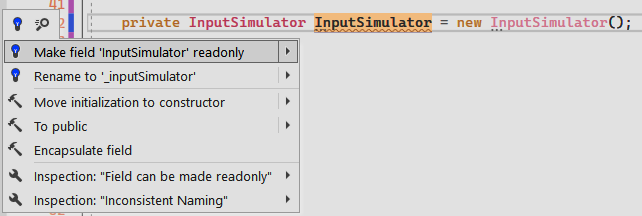
\includegraphics[width=125mm]{images/resharper_refac.png}
	\caption{Refactoring Vorschläge von ReSharper}
	\label{fig:resharper_refactor}
\end{figure}
\FloatBarrier

Alternative Tools für eine derart große Anzahl an unterschiedlichen Sprachen und Funktionen sind aktuell keine auf dem Markt. Kostenlose Alternativen wie \textbf{CodeRush} beschränken sich zumeist auf wenige Sprachen \cite{DocumentationCodeRush}. Allerdings bieten viele IDEs einige dieser Funktionen out of the box an und viele Entwickler arbeiten generell nur mit einer Programmiersprache. Daher können andere, für die jeweilige Programmiersprache geeignete, Tools verwendet werden.
\section{Dokumentation}
\label{sec:documentation_collaboration}
Um ein Projekt mit entwickeltem Code langfristig weiterentwickeln und warten zu können, ist die Dokumentation von diesem notwendig. Als \textit{Softwaredokumentation} ist sämtliche Dokumentation einer Software im Entwicklungsprozess und darüber hinaus zu verstehen. Über den gesamten Entwicklungsprozess werden unterschiedlichste Dokumentationen erstellt. Sie dienen dazu, die Funktionalität, den Nutzen und die Entwicklung der Software für die verschiedenen Stakeholder nachvollziehbar zu machen. Dabei ist auch die Anzahl der Entwickler und die Größe des Projekts zu vernachlässigen. Eine gute Softwaredokumentation ist auch bei nur einem Entwickler essenziell und gewinnt bei größeren Kollaborationen nur noch mehr an Wichtigkeit. Die Softwaredokumentation muss alle wichtigen Fragen der mitwirkenden beantworten können und Aufschluss über die Software geben.  

\begin{quotation}
	\textit{Documentation is highly valued, but often overlooked.}
	\begin{flushright}
		\footnotesize{---opensourcesurvey}
	\end{flushright}
\end{quotation}

Eine großangelegte Umfrage von Open Source\footnote{Softwaregruppierung zur Entwicklung freier Software. (Vgl. https://opensource.com/)} zeigt auf, dass eines der Hauptprobleme bei der Entwicklung freier Software eine unvollständige oder verwirrende Dokumentation ist.
Vielen Entwicklern ist die Wichtigkeit der Dokumentation nicht bewusst. Doch Schlechte Dokumentation kostet Geld \cite{GitHubInc.2017}!

Die Dokumentation geht mit einer erfolgreichen Kollaboration in einem Entwicklerteam einher. Hierbei sind die verschiedenen Entwickler auf Informationen über Schnittstellen, Funktionen einzelner Module und den Änderungsverlauf im Projekt angewiesen.
Für die automatische Dokumentation solcher Informationen stehen dem Entwickler verschiedene intelligente Werkzeuge zur Verfügung. Diese helfen bei der Erstellung der Dokumentationen und verbessern den Entwicklungsprozess. Neben der automatischen Generierung wird auch die Qualität und Konsistenz der Dokumente eingehalten und verbessert. 

Entscheidend ist die Auswahl der Hilfsmittel. Es existiert eine Vielzahl an Hilfsmitteln für verschiedene Arten der Softwaredokumentationen. Bei der Auswahl der Hilfsmittel müssen verschiedene Kriterien, die der Entwicklungsprozess mit sich bringt, berücksichtigt werden. 

\subsection{Allgemeine Konzepte}
\label{subsec:documentation_collaboration_concepts}
In dem Prozess der Softwareentwicklung gibt es viele verschiedene Arten von Dokumentationen. Dabei sind nicht immer alle Arten von Dokumentationen notwendig. Dokumentationen können in verschiedene Bereiche und unterschiedliche Zielgruppen unterteilt werden. Je nach Vorgehen im Entwicklungsprozess und dem Vorhandensein der Zielgruppen, müssen die notwendigen Dokumentationen individuell festgelegt werden. 
Trotz einer Vielzahl an unterschiedlichen Dokumentationsmöglichkeiten lassen sich zwei Hauptkategorien herausarbeiten. 

Bei der \textbf{Projektdokumentation} wird der Fokus auf das Vorgehen, die Methodik, und die Werkzeuge gelegt. Sie ist für die verschiedenen Stakeholder und soll Aufschluss über den Verlauf des Projektes geben. 

Die \textbf{Systemdokumentation} hingegen beschreibt das Produkt. Genauer beschreibt sie, aus was das Produkt besteht und wie es funktioniert und vorgeht. Diese Arte der Dokumentation ist primär für den Entwickler. Gerade bei großen Teams oder späterer Weiterentwicklung ist diese Art der Dokumentation sehr wichtig. 

Das Feld der \textbf{Projektdokumentation} bezieht sich wie beschrieben, auf den Verlauf und die Planung des Entwicklungsprozesses. Hierbei sind die Abläufe projektabhängig und werden Kunden-/Produktspezifisch angepasst. 
Intelligente Werkzeuge können aufgrund der Individualität von Projekten nur begrenzt eingesetzt werden. Die unterstützenden Werkzeuge, die hierbei verwendet werden, sind meist auf die allgemeinen Hilfsmittel einer Projektplanung zurückzuführen. 
Anders verhält sich dies jedoch im Bereich der \textbf{Systemdokumentation}. Dort unterstützen sie bei der Dokumentation des eigentlichen Umsetzungsprozess und bei der Beschreibung des Produkts.

Ein nützliches Werkzeug zur Dokumentation des Aufbaus einer Anwendung ist das \textbf{automatische Generieren von UML-Diagrammen}. UML-Diagramme sind ein wichtiger Bestandteil der Anwendungsdokumentation. Sie dienen in der Softwareentwicklung als ein Standard zur Visualisierung des Systementwurfs \cite{Ambler.2004}. Die UML-Diagramme begleiten den ganzen Entwicklungsprozess der Software. Sie sind sowohl bei der Planung ein wichtiger Bestandteil, als auch bei der dynamischen Umsetzung der Software. Bei der Umsetzung kann der Aufbau in den verschiedenen Stadien visualisiert und so nachverfolgt werden. Die automatische Generierung der Diagramme an sich, ist schon ein wichtiges intelligentes Werkzeug für den Entwickler. Jedoch bieten UML-Diagramme noch mehr Möglichkeiten den Entwicklungsprozess zu erleichtern. So wie ein Diagramm aus dem Qulltext automatisch generiert werden kann, so ist auch Quelltext aus einem Diagramm generierbar. Das bietet dem Entwickler während der Umsetzung die Möglichkeit, Klassen und andere Typen grafisch zu erstellen, zu ändern und zu löschen \cite{TerryG.Lee.2022}.

\textbf{Inline-Kommentare} sind lesbare Kommentare innerhalb des Quelltextes. Sie werden dem Quelltext hinzugefügt, um ihn verständlicher und nachvollziehbarer zu machen. Dies ist wichtig, wenn mehrere Entwickler gemeinsam an einer Anwendung arbeiten. Es kann viele verschiedene Gründe geben, einen Quelltext-Abschnitt oder eine Zeile mit Kommentaren zu versehen. Folgend sind Gründe für Inline-Kommentare aufgelistet.
\begin{itemize}
	\item[(a)] \textbf{Planen und Überprüfen:} Es kann vor dem Beginn der eigentlichen Programmierung anhand von Kommentaren die Umsetzung geplant werden. So kann an den konkreten Stellen, wie bspw. leeren Methoden, ein Kommentar mit der Beschreibung hinterlassen werden. Anhand dieser Beschreibung übernimmt ein Entwickler dann die konkrete Implementierung (siehe \autoref{code:commentexample}).
	\item[(b)] \textbf{Beschreibung des Quelltextes:} Wie im vorherigen Paragraphen beschrieben, ist es wichtig einen schnellen Überblick über den Quelltext zu erhalten. Gerade wenn mehrere Entwickler an dem selben Projekt arbeiten, ist eine Beschreibung am Beginn einer Passage und relevanten Stellen (Methoden, Klassen, ...) sehr hilfreich. 
	\item[(c)] \textbf{Beschreibung des Algorithmus:} Noch wichtiger sind Kommentare bei unübersichtlichen Algorithmen. Auch wenn Quellcode eigentlich selbsterklärend sein soll, ist dies bei komplexen Algorithmen oftmals nicht machbar. Meist ist nicht auf den ersten Blick ersichtlich, was ein Algorithmus bewirkt. Daher kann eine vorhergehende Beschreibung und Kommentierung ausgewählter Stellen sinnvoll sein.
	\item[(d)] \textbf{Verwendung von Ressourcen:} Wird eine externe Ressource verwendet, ist es hilfreich Informationen über den Speicherort und die verwendete Version der Ressource zu hinterlassen. Auch die offiziellen Namen sind bei der Verwendung von Abkürzungen im Quelltext als Kommentare hilfreich. 
	\item[(e)] \textbf{Debugging:} Beim Debugging ist es hilfreich, an bestimmten Stellen Markierungen zu setzen, um den Quelltext während des Debuggings übersichtlich zu halten. 
\end{itemize}

Die Realisierung von Kommentare ist in unterschiedlichen Programmiersprachen unterschiedlich gestaltet. Folgend ist eine Übersicht über einige der verwendeten Token zum Realisieren von Kommentaren dargestellt. 
\begin{table}[]
	\centering
	\begin{tabular}{|l|l|}
		\hline
		\multicolumn{1}{|c|}{Symbol} & \multicolumn{1}{|c|}{Programmiersprache} \\ \hline
		REM    & BASIC, Batch files                                         	\\ \hline
		::     & cmd.exe                                                    	\\ \hline
		\#     & Cobra, Perl, Python, Ruby, Make, Windows PowerShell, PHP   	\\ \hline
		\%     & TeX, Prolog, MATLAB                                        	\\ \hline
		//     & C (C99), C++, C\#, D, F\#, Go, Java, JavaScript, Kotlin			\\ \hline
	\end{tabular}
	\caption{Tokens zu Beginn eines Kommentars in unterschiedlichen Programmiersprachen}
\end{table}
\FloatBarrier

Ein wichtiges Werkzeug, welches Inline-Kommentare ermöglicht und viele Entwicklungsumgebungen unterstützt, ist das verwenden von Tags. Hierbei handelt es sich um Begriffe, die einem Kommentar vorangestellt werden, sodass dieser kategorisierbar ist. Dieses Werkzeug erleichtert das Auffinden von bestimmten Stellen im Quelltext immens. Dabei gibt es verschiedene Tags für unterschiedliche Kategorien. Als Beispiele soll hier \textit{TODO} genannt werden (\autoref{code:commentexample}). Dieser Tag kann an Stellen in einem Kommentar erwähnt werden, an welchen es noch etwas zu implementieren gilt (siehe \autoref{code:commentexample}). Es ist nun dem Entwickler die Möglichkeit gegeben, sich alle Kommentare mit diesem Tag auflisten zu lassen. Dadurch hat er eine schnelle Übersicht, an welchen stellen Änderungen notwendig sind und kann automatisch zu diesen navigieren. Durch den Inhalt des Kommentars, ist auch auf einen Blick zu erkennen, was zu tun ist. 
Neben dem genannten \textit{TODO} Schlüsselwort gibt es noch weitere typische Tags, die folgend aufgelistet sind \cite{JillReinauer.2016}: \textit{BUG, DEBUG, FIXME, TODO, UNDONE}.
\begin{lstlisting}[caption={Beispiel von Inline-Kommentaren}, label=code:commentexample]
	//Konstruktor der Klasse 
	public Program(int a, int b){
		
		//TODO: addiere a + b
		
	}
\end{lstlisting}
\FloatBarrier
Eine weitere Möglichkeit welche Inline-Kommentare bieten, ist die automatische Generierung einer Dokumentation des Quelltextes. Durch Einhaltung einer bestimmten Syntax, kann im Nachgang eine vollständige Dokumentation mit Beschreibungen der Klassen, Methoden und Parameter erstellt werden. Diese wird in der Regel als HTML-Dokument erzeugt und kann somit einfach freigegeben werden. Dies kann mit der UML-Diagrammerzeugung verglichen werden, wobei es sich hier nur um textuelle Beschreibungen handelt. Es stehen mehr die einzelnen Aufgaben der Klassen und Methoden im Vordergrund, als deren Zusammenhang. 

Als Syntax der Kommentare können unterschiedliche Formate vorgegeben sein. Je nach verwendetem Generator kann es auch eine individuelle Syntax und Semantik des Generators sein. Ein bekanntes Format was auch genutzt wird, ist das XML-Format. Mit diesen verschiedenen Standards lassen sich Beschreibungen zu Elementen und Kommentaren erstellen, mit denen anschließend automatisch eine Dokumentation generiert werden kann. 

\subsection{Marktanalyse}
\label{subsubsec:diagramanalyses}
Bezüglich der \textbf{Erzeugung von UML-Diagrammen} sind viele verschiedene Werkzeuge auf dem Markt vertreten. In den meisten kommerziell genutzten Entwicklungsumgebungen ist ein UML-Generator standardmäßig vorhanden. Dies unterscheidet sich aber je nach Entwicklungsumgebung. In den bekannten Entwicklungsumgebungen Visual Studio von Microsoft (\autoref{fig:uml_2}) und Intelij von JetBrains sind UML-Generatoren vorhanden. Bei Visual Studio ist der UML-Generator auch in der kostenlosen Community Version enthalten. 

Zudem unterstützt nur Visual Studio das Erstellen und Bearbeiten von Quelltext mit Hilfe der UML-Diagramme. Dies hat in eigens durchgeführten Versuchen sehr gut funktioniert. Es konnten Anwendungsstrukturen mit Hilfe der UML-Diagramme erstellt werden. Auch das nachträgliche Umbenennen von Klassen und Methoden hat hervorragend funktioniert \cite{TerryG.Lee.2022}\cite{JetBrains.2022}.
\begin{figure}
	\centering
	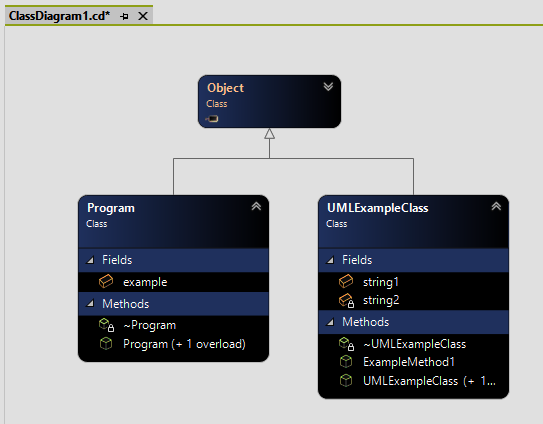
\includegraphics[width=6cm]{images/uml_vs.png}
	\caption{Ein von Visual Studio generiertes UML-Diagramm}
	\label{fig:uml_2}
\end{figure}
\FloatBarrier
Ein Werkzeug, welches unabhängig von der Programmierumgebung arbeitet, ist Doxygen. Es handelt sich um das Standard Werkzeug für die automatische Dokumentationsgenerierung. Einige der unterstützten Programmiersprachen sind C++, C, Objective-C, C\#, PHP, Java und Python \cite{Doxygen.2022}. 

Zur \textbf{Inline-Dokumentation} kann dagegen beispielhaft JavaDoc verwendet werden. Dieses ist in Intelij standardmäßig im Einsatz und verfügbar (siehe \autoref{code:codedescription}). 
\begin{lstlisting}[caption={Beispiel von Inline-Kommentaren}, label=code:codedescription]
	/**
	* Beschreibung der Methode
	* @param integer1 Beschreibung Parameter 1
	* @param integer2 Beschreibung Parameter 2
	* @return Beschreibung des zu retunierenden Wert
	*/
	public static String test(int integer1, int integer2){
		
		return "foo";
	}
\end{lstlisting}
\FloatBarrier
Die in \autoref{code:codedescription} verwendeten Kommentare erzeugen \autoref{fig:htmlBeschreibungMethode}. 
\begin{figure}
	\centering
	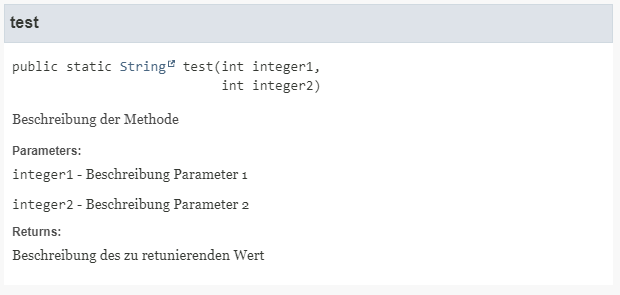
\includegraphics[width=10cm]{images/htmlBeschreibungMethode.png}
	\caption{Automatisch generierte Übersicht einer Java-Methode \autoref{code:codedescription}}
	\label{fig:htmlBeschreibungMethode}
\end{figure}
\FloatBarrier
Dennoch gibt es auch in diesem Feld weiter Anbieter, die eine Dokumentationserzeugung aus Inline-Kommentaren erlauben. Um den erwähnte XML-Standard aufzugreifen, ist hier Visual Studio zu erwähnen. In Visual Studio ist ein Bordmittel integriert, mit welchem sich die XML-Kommentare in eine HTML-Dokumentation wandeln lassen. Dazu gibt es verschiedene Schlüsselwörter, welche zur Beschreibung verwendet werden. So wird zum Beispiel das Schlüsselwort \textit{<summary>} zum Definieren einer Beschreibung eines bestimmten Elements verwendet werden. Des Weiteren können Parameter mit Kommentaren und Anmerkungen versehen werden. Dies geschieht mit dem Schlüsselwort \textit{<param name="nameDesParameters">Beschreibung des Parameters</param>}. 

Beim Verwenden der zwei Werkzeuge ist schon zu erkennen, dass sich das Prinzip nur leicht unterscheidet. Die Syntax und Semantik, mit welchen die Kommentare anzugeben sind, unterscheiden sich zwar im Format, jedoch ähneln sich die erzeugten Dokumentationen im Stil und Aufbau sehr. 

Doxygen, wie schon erwähnt (\autoref{subsubsec:diagramanalyses}), begrenzt sich nicht nur auf die UML-Diagrammerzeugung, sondern bietet auch in diesem Feld eine Lösung. Es kombiniert die Felder und gibt in der erzeugten Dokumentation sowohl die UML-Diagramme, als auch die einzeln definierten Beschreibungen an. Hierbei setzt Doxygen auf eigens definierte Befehle. Es gibt Befehle der Form \textit{\textbackslash Befehl} welche die Art des Kommentars beschreiben. Aber auch die erzeugte Dokumentation von Doxygen ähnelt den erwähnten Werkzeugen sehr. 

Eine Alternative, die für viele Programmiersprachen verwendet werden kann, ist Natural Docs. Natural Docs unterstützt 21 Programmiersprachen und ist folglich an keine Programmierumgebung gebunden. Dabei bindet sich Natural Docs wie Doxygen an keinen Stadard, sondern definiert seine eigenen Befehle zum Kommentieren.

Als ein bekanntes Beispiel einer automatisch generierten Dokumentation, bietet Oracle eine Dokumentation von Java\footnote{Vgl.: https://docs.oracle.com/javase/7/docs/api/overview-summary.html}. Dabei sind die einzelne Methoden, Klassen und Schnittstellen von den verschiedenen Java-Versionen dokumentiert.  
%% ggf. noch gituml falls ich noch was brauche - FW 15.11
%% + visual paradigme oder objectiFi

\subsection{Nutzen und Risiken}
Durch Werkzeuge zur Dokumentation werden Schritte des Prozesses automatisiert. Somit wird dieser weniger Fehleranfällig und einfacher anzuwenden. Durch die nun einfache Dokumentation sind Entwickler eher geneigt, ihren Code tatsächlich zu dokumentieren. Somit wird beispielsweise bei der Verwendung von dokumentierten Methoden klar, was die jeweilige Methode im Detail macht und worauf ggf. geachtet werden muss. Dies ist besonders bei großen Projekten wichtig, in welchen aufgrund getrennter Entwicklung regelmäßig fremde Methoden verwendet werden. So wird direkt bei den Vervollständigungsvorschlägen (siehe \autoref{sec:codecompletion}) die Inline-Dokumentation angezeigt. Außerdem müssen Diagramme nicht weiterhin von Hand erzeugt werden, sondern sind einfach exportierbar, sowie importierbar. 

Trotz aller Vorteile muss jedoch immer ein Mittelmaß gefunden werden. Gute Dokumentation ersetzt nicht \textit{Clean Code}, also beispielsweise die Verwendung von sinnvollen Namen. Außerdem muss darauf geachtet werden, dass Dokumentation auch bei Änderungen im Code aktuell gehalten wird. Ansonsten unterscheidet sich die Beschreibung von der tatsächlichen Funktionalität. Nicht zuletzt sollten Kommentare kurz und verständlich anstelle von lang und unübersichtlich sein. Ansonsten wird unnötig viel Zeit darauf verwendet und es fehlt eine einfache, schnelle Verständlichkeit. Eine übertriebene Nutzung der Kommentarfunktion kann den Quellcode sogar weniger leserlich machen. 

Bezüglich von Diagrammerzeugung muss außerdem erwähnt werden, dass gewisse Besonderheiten ggf. nicht automatisch in ein Diagramm übersetzt und somit manuell nachgebessert werden müssen. Erwähnenswert sind außerdem die möglicherweise anfallenden Kosten. Dies betrifft auch Werkzeuge zur Diagrammerzeugung aus Quelltexten wie in der Marktanalyse ersichtlich ist (\autoref{subsubsec:diagramanalyses}). 
\section{Kollaboration}
Ein weiteres wichtiges intelligentes Werkzeug, welches sich im Bereich der Dokumentation und Kollaboration befindet, ist die Versionsverwaltung. Diese ermöglicht während des gesamten Projektes die Zusammenarbeit mehrerer Personen, Versionierung, als auch Dokumentation der Änderungen. Große Projekte sind undenkbar ohne Versionsverwaltung.

\subsection{Allgemeines Konzept}
\label{subsubsec:vc}
Die Versionsverwaltung ist gerade bei Kollaborationen mehrerer Entwickler essenziell. Sie wird zum Erfassen von Änderungen an Dateien und Dokumenten verwendet. Eine Versionsverwaltung bietet einige Vorteile. Darunter zählen Transparenz, Übersicht, Nachverfolgbarkeit, Zusammenarbeit mehrerer Entwickler und Identifikation. All dies führt zu einer Effizienzsteigerung. Dabei muss es sich bei zu verwaltenden Daten nicht, wie weitläufig bekannt, nur um Quelltexte handeln. Eine Versionsverwaltung kann auch für Text- oder Tabellendokumente verwendet werden. Im Folgenden wird zwar überwiegend auf die Verwaltung von Quelltexten eingegangen, dennoch soll erwähnt werden, dass eine Versionsverwaltung in den verschiedensten Projektbereichen eingesetzt werden kann. Dies gibt den Entwicklern die Möglichkeit, Änderungen nachzuverfolgen und gegebenenfalls rückgängig zu machen. Des Weiteren lassen sich vielseitige Statistiken über die getätigten Änderungen erstellen. Weitere Hauptaufgaben einer Versionsverwaltung sind Protokollierung, Wiederherstellung, Archivierung, Koordinierung und das gleichzeitige entwickeln mehrere Zweige. 
\begin{comment}
	Ein Hautpelement einer Versionsverwaltung ist das Ermöglichen von continuous integration, continuous delivery (CI/CD). CI/CD ist eine Methode, welche die Automation von verschiedenen Stadien einer Anwendungsentwicklung ermöglicht. 
	
	Ein weitere Möglichkeit die das Werkzeug der Versionsverwaltung durch eine Zentrale Lagerung der Dateien ermöglicht, ist  continuous integration/continuous delivery (CI/CD). 	
\end{comment}
Für die genannten Aufgaben verfügt jede Versionsverwaltung über fünf Basisaktionen, welche diese Aufgaben ermöglichen. 
\begin{itemize}
	\item[(a)] \textbf{Add}: Fügt Dateien zur Versionsverwaltung hinzu.
	\item[(b)] \textbf{Remove}: Entfernt Dateien aus der Versionsverwaltung.
	\item[(c)] \textbf{Commit}: Veröffentlicht vorgenommene Änderungen. 
	\item[(d)] \textbf{Revert}: Setzt die aktuelle Version auf den letzten veröffentlichten Stand zurück. 
	\item[(e)] \textbf{Branch}: Erzeugt einen neuen Zweig aus einem bestehend Zweig. 
	\item[(f)] \textbf{Merge}: Fügt zwei Zweige zusammen und passt Differenzen an. 
\end{itemize}
Darüber hinaus gibt es noch viele weitere Möglichkeiten, die ein Versionsverwaltungssystem besitzen kann. Die genannten Möglichkeiten sind die Grundlagen, die Versionsverwaltungssysteme beherrschen \cite{Davis.2020}. Die Möglichkeiten die dem Entwickler dadurch gegeben werden, sind im Entwicklungsprozess sehr wichtig und werden in den meisten Projekten eingesetzt. Auf Quelltexte bezogen, bietet die zentrale Lagerung der Quelltext-Dateien noch weitere Vorteile. 

Wie in einem Verwaltungssystem üblich, können verschiedene Rollen vergeben werden. Diese ermöglichen die Vergabe von Freigaben und somit eine Rechteverwaltung. Dadurch ist die Möglichkeit gegeben, Änderungen erst nach einer Absprache und/oder Korrektur freizugeben.
Eine weitere Hauptaufgabe, welche Versionsverwaltungssysteme ermöglichen ist die Integration spezieller Abläufe bei der Aktualisierung der Version. So können festgelegte Buildvorgänge, Sicherungen oder verschiedenen Tests der Anwendung durchgeführt werden. 

\subsection{Martkanalyse}
\label{subsubsec:vcanalyze}
Auf dem Markt gibt es unzählige Versionsverwaltungssysteme mit verschiedenen Schwerpunkten für verschiedensten Betriebssysteme. Darunter sind zum Beispiel \textit{Git}, \textit{Subversion (SVN)} und \textit{Concurrent Version System (CVS)}. Das wohl bekannteste Versionsverwaltungssystem ist Git. Git unterscheidet sich insofern von anderen, als das es ein verteiltes System ist. Das bedeutet, dass jede Kopie des Verzeichnisses die gesamten Metadaten inklusive des Änderungsverlaufs enthält und so ein eigenständiges und abgekapseltes Verzeichnis bildet. Git ist kostenlos nutzbar und ein OpenSource-Projekt. Gleiches gilt für Subversion, welches wie git eine große Bekanntheit genießt und von der Apache Software Fundation entwickelt wird. Das Ziel von Subversion ist es, der Nachfolger des in der Vergangenheit sehr bekannten Concurrent Version System zu sein. 

Mit 94 Millionen Nutzern ist GitHub\footnote{https://github.com/} ein sehr bekanntes, auf Git basierendes, Versionsverwaltungssystem im Internet. An diesem Beispiel ist sehr gut zu erkennen, welche weiteren Möglichkeiten eine Versionsverwaltung bietet. Neben Integration der oben genannten Standard-Werkzeugen einer Versionsverwaltung, bietet Github noch viele Erweiterungen rund um die Versionsverwaltung. So können Teams mit Dashboards und verschiedenen Statistiken zum Projekt arbeiten. Auch können verschiedenste Automationen eingepflegt werden, welche den Entwicklungsprozess erleichtern. Bei größerem Interesse kann bei einer Recherche das Stichwort CI/CD  oder DevOps unterstützen. 

\subsection{Nutzen und Risiken}
\label{subsec:documentation_collaboration_risks}
Durch die dadurch VCS entstehenden Möglichkeiten ist eine große Effektivitätssteigerung in Projekten möglich. Sie vereinfachen die Zusammenarbeit in großen Teams und Kollaborationen. Die Werkzeuge sind in den unterschiedlichsten Ausprägungen in vielen Firmen vertreten und werden von vielen Entwicklern schon als Standard angesehen. Zudem sorgen die Möglichkeiten zur Nutzung verschiedener Branches, das Mergen und die Dokumentation der Änderungen generell für eine höhere Sicherheit des Codes. Fehler können schnell identifiziert werden, eine lauffähige Version ist immer vorhanden und es kann unabhängig von anderen entwickelt werden. 

Ein Risiko, welches die Werkzeuge dennoch bieten ist, dass sie über ihre Maße angewandt werden. Auch bei der Versionsverwaltung ist dies ein Thema. Viele Anbieter bieten über die Standardmöglichkeiten einer Versionsverwaltung hinaus Werkzeuge an. Diese sind jedoch nicht immer erforderlich. Ein weiterer Punkt ist, dass die meisten Werkzeuge für den kommerziellen Einsatz in Unternehmen kostenpflichtig sind. Die genannten Werkzeuge werden meist auf Unternehmensinterne Daten angewandt. Deshalb ist auch der Datenschutz ein sehr wichtiger Punkt, welcher nicht vernachlässigt werden sollte. Hierfür bieten die genannten Anbieter zwar Lösungen, wie zum Beispiel die Werkzeuge Unternehmensintern zu hosten, dennoch sollte der Datenschutz nicht vernachlässigt werden. 

\section{Schluss}
\label{sec:schluss}
Abschließend soll in einer kurzen Zusammenfassung die Arbeit zusammengefasst und die Erkenntnisse zentral gesammelt werden. Danach folgt mit den durch die Arbeit erlangten Erkenntnisse ein Ausblick in die Zukunft von intelligenten Werkzeugen zur Softwareentwicklung. 

In der vorliegenden Arbeit wurden wichtige intelligente Werkzeuge zur Softwareentwicklung aufgezeigt. Dazu wurden die theoretischen Grundlagen der einzelnen Werkzeuge genauer aufgezeigt und die in einer Marktanalyse ausgewählte Werkzeuge, welche in der Praxis Anwendung finden, näher analysiert. Abschließend wurden der Nutzen und die möglichen Risiken der einzelnen Werkzeuge evaluiert. Die ausgewählten Werkzeuge, welche vorgestellt wurden, erleichtern den Entwicklungsprozess in essenzieller Weise und gestalten die Arbeit effizienter. Genauer wurden intelligente Werkzeuge zur Codevervollständigung, Codegenerierung, Analyse, Refactoring, Dokumentation und Kollaboration vorgestellt. 
Bei der Marktanalyse ist aufgefallen, dass es eine Vielzahl von Anbietern intelligenter Werkzeuge gibt. Zwar gibt es teilweise sprachübergreifende Werkzeuge, dies ist allerdings nicht immer der Fall. Manchmal kann daher eine gesonderte Analyse bezüglich verwendetem Technologie-Stack sinnvoller sein. 
Des Weiteren ist ersichtlich, dass bestimmte Entwicklungsumgebungen die genannten Werkzeuge bereits implementieren. Daher muss in diesen Fällen nicht auf eine externe Lösung gesetzt werden. Dies spiegelt aber auch die Akzeptanz und Wichtigkeit dieser Werkzeuge bei der Entwicklung wieder. 
Die Analysen zeigen, dass jedes der vorgestellten intelligenten Werkzeuge den Entwicklungsprozess effizienter gestaltet. Die genannten Gefahren dabei sind meist, dass sich der Entwickler zu sehr auf die Werkzeuge verlässt und diese nicht hinterfragt. Daher sind die Werkzeuge aufgrund ihrer Effizienzsteigerung zu empfehlen, jedoch sollten Entwickler ihnen nicht blind vertrauen und dennoch die Ausgabe selbst kontrollieren. 

Wie aus der Arbeit hervorgeht, sind viele intelligente Werkzeuge jetzt schon in der Softwareentwicklung etabliert. Auch an den Nutzerzahlen der einzelnen Werkzeuge, die in den Marktanalysen genannt wurden, lässt sich dies aufzeigen. Dennoch gibt es auch andere Meinungen. Gerade wie sich in der Marktanalyse zum Thema Refactoring (\autoref{subsec:Refactoring_analyse}) herausgestellt hat, ist das Vertrauen zu gewissen Werkzeugen noch nicht vollständig hergestellt und bedarf noch gewisser Erfahrung. Dennoch betrifft dies nicht alle Werkzeuge. 
Das Themengebiet der vollständig auf künstliche Intelligenz basierten Werkzeuge bietet in Zukunft noch viel Entwicklungspotenzial. Wie zum Beispiel das Werkzeug der Codegenerierung \autoref{sec:codecompletion} zeigt, bietet es immense Möglichkeiten den Entwicklungsprozess zu erleichtern oder gar zu automatisieren. Von einer vollständigen Automatisierung ist hier aber in absehbarer Zeit nicht zu reden. Dennoch entwickelt sich das allgemeine Feld der künstlichen Intelligenz rasant und die Prognosen sind hierzu nur bestätigend \cite{statista.2022}. Deshalb ist davon auszugehen, dass auch die intelligente Werkzeuge immer mehr von dieser Technik profitieren und dadurch weiterentwickelt werden. 
Wie die Arbeit des Weiteren aufzeigt ist das Themengebiet hoch aktuell und sehr wichtig. So werden auch in Zukunft noch einige interessante Neuerungen und Weiterentwicklungen in diesem Bereich stattfinden. 

\printbibliography
\end{document}
